\documentclass[a4paper, 12pt, twoside]{article}
\usepackage{ae,aecompl}
\usepackage[T1]{fontenc}
\usepackage[utf8]{inputenc}
\usepackage[ngerman]{babel}
\usepackage{textcomp}
\usepackage{anysize}
% left right up down
\marginsize{3.2cm}{2.8cm}{2cm}{2cm}
\usepackage{setspace}
\setstretch{1.2}
\frenchspacing
\usepackage{chemfig}
\usepackage{gensymb}
\usepackage{fancyhdr}
\usepackage{enumerate}
\usepackage{amsmath}
\usepackage{upgreek}
\usepackage{indentfirst}
\usepackage{sidecap}
\numberwithin{equation}{section}
\numberwithin{figure}{section}
\numberwithin{table}{section}
\usepackage{multicol}
\usepackage{float}
\setcounter{tocdepth}{1}
\pagestyle{empty}
% uncomment for hyperlinks
\usepackage{xcolor}
\usepackage[colorlinks = true,
            linkcolor = red,
            urlcolor  = blue,
            citecolor = blue,
            anchorcolor = blue]{hyperref}



\title{Laborpraxis für physikalische Chemie}
\author{\emph{verfasst von:} \\ Barna Kovács \\ Sándor Kunsági-Máté \\ András Kiss \\ Géza Nagy \\ \\ \emph{übersetzt von:} \\ András Kiss \\ \\ \\ \\ \\ \\
\includegraphics[width=0.2\textwidth]{fig/pte_logo.eps} \\
Abteilung für allgemeine und physikalische Chemie \\ Universität Pécs}

\begin{document}

\clearpage\maketitle
\thispagestyle{empty}
\newpage 
\tableofcontents
\newpage

%\setcounter{section}{1}
\section{Bestimmung des Dissoziationskonstanten von schwachen Säuren mit Leitfähigkeitsmessung}
\subsection{Theoretische Grundlage}

Elektrischer Widerstand ist eine Eigenschaft des Materials. Nach dem ohmschen Gesetz ist zwischen den Materialen durchpliessenden Stromstärke ($I$) und den Strom erstellenden Spannung ($U$) ein gerades Verhältniss.


\begin{equation}
\label{eq:ohm}
	U
	=
	I
	\cdot
	R
\end{equation}

wo der Verhältnissfaktor $R$ als Widerstand des Materials genannt wird, dessen Einheit ist der ohm ($\ohm$).
An spezifischer Widerstand verstehen wir den Quotient von der Spannung die zur Erstellung von ein 1 A (Amper) starken Strom nötig ist und den Strom von 1 A. %%%

In der Elektrochemie ist es aus mehreren Hinsichten bevorzüglich, wenn wir den Reziprok von oben genannten Einheiten benutzen: den Reziprok vom Widerstand nennen wir Leitfähigkeit (Enheit ist Siemens, S$ = 1 / \ohm$), den Reziprok von spezifischen Widerstand nennen wir spezifischen Leitfähigkeit (Einheit ist S/cm).
An spezifischen Leitfähigkeit von Elektrolytlösungen ($\kappa$) nennen wir die Leitfähigkeit von Elektrolytlösung zwischen zwei Leitern von erste Klasse die 1 cm entfernt von einander sind und eine Fläche von 1 cm$^2$ haben.
Die spezifische Leitfähigkeit ist abhängig von der materiellen Qualität, von der Konzentration und von der Temperatur des Elektrolyten.
An molar spezifische Leitfähigkeit ($\Lambda _m$) verstehen wir den Quotient von der spezifischer Leitfähigkeit und der Konzentration.

\begin{equation}
\label{eq:lambdam}
        \Lambda_m
        =
        \frac
		{\kappa 1000 }
		{c}
	=
	\kappa V
\end{equation}

wo $c$ ist Konzentration (mol$\cdot$dm$^{-3}$), und $V$ ist Verdünnung.

Die molare Leitfähigkeit der unendlich verdünnten Lösung wird molare Grenzleitfähigkeit genannt ($\Lambda _m^0$).
Nach \emph{Kohlrausch}\footnote{Friedrich Wilhelm Georg Kohlrausch war ein deutscher Physiker und Physikochemiker.} summiert sich die Leitfähigkeit von Anionen und Kationen in dünnen Lösungen von starken Elektrolyten. 

%Kohlrausch szerint erős elektrolitok híg oldataiban az anionok és kationok moláris fajlagos vezetőképessége összeadódik.

\begin{equation}
\label{eq:kohlrausch2}
	\Lambda _m^0
	=
	\lambda _a^0 \nu _a z_a + \lambda _k^0 \nu _k z_k
%	/1000
\end{equation}

wo $z_a, z_k$ sind die Ladung, $\nu _a, \nu _k$ sind die stöchiometrischen Faktoren, und $\lambda _a^0, \lambda _k^0$ sind die Grenzleitfähigkeiten von Anionen ($a$) und Kationen ($k$).

Die Leitfähigkeit von dünnen Elektrolyten werden bezeichnet als:

\begin{equation}
\label{eq:lambdam}
        \lambda_c
        =
        \alpha
	\lambda_0
\end{equation}

wo $\alpha$ den Dissoziationsgrad, $\lambda _0$ die Grenzleitfähigkeit bedeutet.

Der Dissoziationskonstant einer schwachen Säure ist berechenbar wenn die Konzentrazion und der Dissoziationsgrad bekannt ist:

\begin{equation}
\label{eq:kd}
        K_d
        =
        \frac{\alpha^2 c}{1-\alpha}
\end{equation}

Es ist aber erwähnenswert, dass nach dem Debye--Hückel--Grenzgesetz, der Dissoziationkonstant $K_d$ bei konstanter Temperatur auch von Permittivität abhängig ist.

Wenn wir die nach $\alpha$ geordnete Form der Gleichung \ref{eq:lambdam} in die vorherige Gleichung substituieren, dann kommen wir auf den von \emph{Ostwald}\footnote{Friedrich Wilhelm Ostwald war ein deutsch-baltischer Chemiker und Philosoph.} bestimmten Zusammenhang der Dissoziation von schwachen Elektrolyten. Dieser Zusammenhang ist als \emph{Ostwaldsche Verdünnungsgesetz} bekannt:

\begin{equation}
\label{eq:ostwald}
        K_d
        =
        \frac{\lambda_c^2 c}{\lambda_0^2 - \lambda_0\lambda_c}
\end{equation}

Das bedeutet, dass wir dem K$_d$ mit Leitungsfähigeitsmessen bestimmen können.
$\lambda_c$ ist direkt messbar, wärend $\lambda_0$ mit der umgeordneten Form von Gesetz \ref{eq:ostwald} bestimmbar ist:

\begin{equation}
\label{eq:ostwald2}
        \frac{1}{\lambda_c}
        =
	\lambda_c
	c
	\frac{1}{K_d \lambda_0^2}
	+\frac{1}{\lambda_0}
\end{equation}

Wenn wir $1/\lambda_c$ als Funktion von $\lambda_c c$ ($= \kappa$) erzeichnen, bekommen wir eine Gerade mit ein Ordinatenabschnitt von $1/\lambda_0$. 
Wenn $\lambda_c$ und $\lambda_0$ bekannt ist, können wir auch den Wert $K_d$ bestimmen.
Bei der Ausführung der Messungen sind folgende Dingen zu beachten: 

\begin{enumerate}[(a)]
\item Neben der gelösten Substanz trägt das Lösungsmittel zur gemessenen Leitfähigkeit der Lösung bei.
Mit eine zugäblichen Messung bestimmen wir die Leitfähigkeit der Lösungsmittel ($G_{\text{Lösungsmittel}}$), und diesen Wert subtrahieren wir aus dem Leitfähigkeit der Lösung.

\item In der Praktik messen wir die Leitfähigkeit nicht mit dem Messgerät aus der Definition von spezifischen Leitfähigkeit, sondern mit einer einfacher, nutzbarer Zelle mit abweichender Geometrie.
Den Unterschied berücksichtigen wir mit der Kalibrationparameter genannt als Zellenkonstant $C$.
Der Zellenkonstant bezeichnet die Verbindung zwischen der Lösung mit einen bekannten spezifischen Leitfähigkeit ($\kappa_{ref}$) und mit der Messzelle gemessene Leitfähigkeit($G_{\text{gemessene}}$). Die Einheit von Zellenkonstant ist m$^{-1}$ oder cm$^{-1}$.

\begin{equation}
\label{eq:c}
	C
	=
	\kappa_{\text{ref}}/G_{\text{measured}}
\end{equation}

\end{enumerate}

Aufgrund dessen bekommen wir den Beitrag der Lösung zur Leitfähigkeit folgender Weise: $\kappa_{\text{korr}} = (G_{\text{Lösung}} - G_{\text{Lössungsmittel}})C$,
wo $\kappa_{\text{korr}}$ ist ein korrigierte Wert von der spezifischen Leitfähigkeit von gelösste Substanz durch den Zellenkonstant und durch die spezifischen Leitfähigkeit des Lösungsmittels. 
$C$ ist der Zellenkonstant, nicht zu verwechseln mit der Konzentration, was mit kleinem $c$ bezeichnet wird.
So bekommen wir die molare Leitfähigkeit der Lösung folgenderweise:

\begin{equation}
\label{eq:c}
        \lambda
        =
        \kappa_{korr}
	V
\end{equation}

wo $V$ verdünnung bedeutet.

\begin{figure}[h!]
\centering
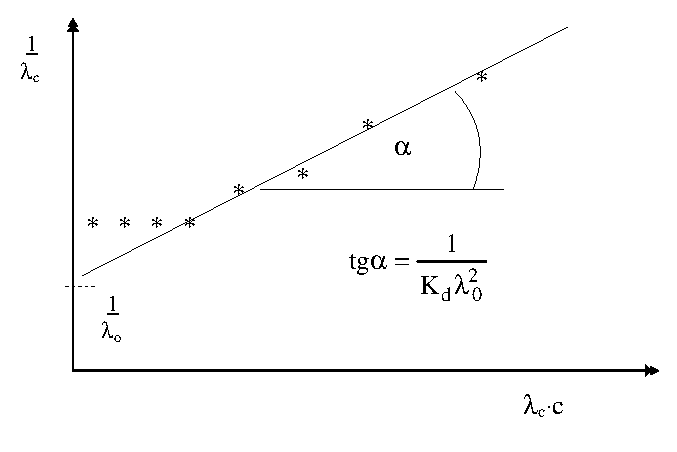
\includegraphics{fig/lambda0.eps}
\caption{Bestimmen der molaren Grenzleitfähigkeit ($\lambda_0$).}
\label{fig:}
\end{figure}

\subsection{Beschreibung des Praktikums}

Spülen Sie die Elektrode von Konduktometer (Leitfähigkeitsmessgerät) vier--fünfmal mit vollentzalztes Wasser, dann mit doppelentsalzten Wasser ($\kappa$ < 1 $\upmu$S/cm), was Sie von der technischen Hilfsperson bekommen.
Richten Sie eine Alkohollösung von 20 v/v\% Volumenkonzentration zu, mit dem Alkohol (Metanol, Etanol oder Propanol) was Ihnen der Praktikumleiter anbietet.
Richten Sie zweierlei Lösungen aus der bekommenen 1 mol$\cdot$dm$^{-3}$ Schwachsäure Stammlösung:
Nehmen Sie zwei trockene 100 cm$^3$ Messkolben und geben Sie mit der Pipette 2--2 cm$^3$ Stammlösung rein.
Dann füllen Sie den einen Messkolben mit doppelvollentsalztes Wasser, den anderen mit 20 v/v\% Alkohollösung bis zur Eichmarke.
Messen Sie die Leitfähigkeit in einen Messzylinder.
Füllen Sie erst die wasserverdünnte Lösung in den Messzylinder, und messen Sie die Leitfähigkeit.
Nachdem saugen Sie 25 cm$^3$ aus dieser Lösung und entlehren Sie sie in einen 50 cm$^3$ grossen Messkolben und füllen Sie bis zur Eichmarke mit doppelvollentsalztes Wasser.
Nach der sorgfeltigen Spülung der Elektrode, wiederholen Sie die Messungen.
Die Prozedur (Verdünnung, Spülung, Messung) wiederholen Sie noch dreimal--viermal.
Wiederholen Sie die ganze Prozedur mit den alkoholverdünnten Lösungen genauso, durch Spülung und Verdünnung mit Alkohollösung.

Bei jeder Messung notieren Sie die Temperatur der Lösung, was das Messgerät anzeigt.

Letzendlich, messen Sie die Leitfähigkeit von dem gebrauchten entzaltzten Wasser, und dem Alkohollösung vomit Sie die Messergäbniste korrigieren müssen.
Nachdem messen Sie die Leitfähigkeit von 0.1 oder 0.01 M KCl Lösung, damit Sie den Zellenkonstant bestimmen.

Abbildung \ref{fig:vez} zeigt das Schema von dem Leitfähigkeitsmesszellen.
In die Lösung tauchen wir zwei geometrischrichtig definierte indifferente Elektroden, und messen die entstehende Spannung. 
Um die elektrische Polarisation zu vermeiden, benutzt das Messgerät Wechselstrom. 

\begin{figure}
\centering
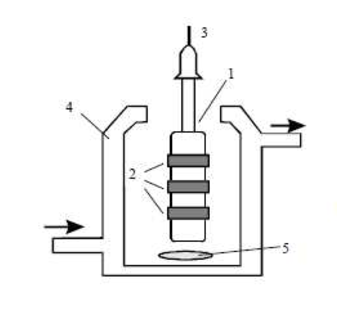
\includegraphics{fig/cond.eps}
\caption{Schema von dem Leitfähigkeitmesszellen. 1 - Elektroden, 2 - Platinum, 3 - elektrische Verbindung, 4 - doppelwandiger Behälter, 5 - Magnetrührer.}
\label{fig:vez}
\end{figure}

\subsection{Auswertung der Messungen}

\begin{enumerate}
\item Rechnen Sie der Zellenkonstant.
Die Messergäbnisse fassten Sie in eine Tabelle:

\begin{table}[!h]
\centering
\begin{tabular}{|c|c|c|c|c|c|c|c|}
\hline
c (mol $\cdot$ dm$^{-3}$) & G$_{\text{gemessene}}$ & $\kappa_{\text{korr}}$ (S $\cdot$ cm$^{-1}$) & $\lambda_c$ & $1/\lambda_c$ & $\lambda_c c$ & $\alpha$ & $K_d$ \\
\hline
... & ... & ... & ... & ... & ... & ... & ... \\
\end{tabular}
\label{table:vez}
\end{table}

\item Bestimmen Sie grafisch den $\lambda_0$ Wert. Mit diesem bekommenen Ergebnissen ($\lambda_c, \lambda_0$) rechnen Sie die $\alpha$ und $K_d$ auf jede Konzentration. 

\end{enumerate}

\newpage
\fancyhead[LE,RO]{Appendix A -- Ionic conductivity at infinite dilution}
\fancyhead[LO,RE]{\thesection}
\fancyfoot[LE,RO]{\thepage}
\fancyfoot[RE,LO]{\emph{Physical chemistry lab. practice for pharmacy students}}

\section*{Appendix A -- Ionic conductivity at infinite dilution}
\addcontentsline{toc}{section}{Appendix A -- Ionic conductivity at infinite dilution}
The following table includes the molar ionic conductivities at infinite dilution for certain ions, that are necessary for evaluations in certain practices. The values refer to aqueous solutions at 25 $\celsius$.

\begin{table}[h!]
\centering
\caption{Molar ionic conductivity at infinite dilution. Source: CRC Handbook of Chemistry and Physics 76th edition, David R. Lide editor in chief, 1995-1996 ISBN: 0-8493-0476-8.}
\label{table:conductivities}
\vspace{5mm}
\begin{tabular}{l|c}
%\hline
                        Ion \hspace{2cm} & $\lambda^0_\pm$, $\cdot$10$^{-4}\cdot$m$^2 \cdot$S$\cdot$mol$^{-1}$\\
                      \hline


Ag$^+$ \dotfill & 61.9 \\
1/3 Al$^{3+}$ \dotfill& 61 \\
1/2 Ba$^{2+}$\dotfill& 63.6 \\
1/2 Be$^{2+}$\dotfill& 45 \\
1/2 Ca$^{2+}$\dotfill& 59.47 \\
1/2 Cd$^{2+}$\dotfill& 54 \\
1/3 Ce$^{3+}$\dotfill& 69.8 \\
1/2 Co$^{2+}$\dotfill& 55 \\
%1/3 [Co(NH$_3$)$_6$]$^{3+}$\dotfill& \\
%1/3 [Co(en)$_3$]$^{3+}$\dotfill& \\
%1/6 [Co$_2$(trien)$_3$]$^{6+}$\dotfill& \\
%1/3 Cr$^{3+}$\dotfill& \\
%Cs$^+$\dotfill& \\
1/2 Cu$^{2+}$\dotfill& 69.3 \\
%D$^+$\dotfill& \\
%1/3 Dy$^{3+}$\dotfill& \\
%1/3 Er$^{3+}$\dotfill& \\
%1/3 Eu$^{3+}$\dotfill& \\
1/2 Fe$^{2+}$\dotfill& 54 \\
1/3 Fe$^{3+}$\dotfill& 68 \\
%1/3 Gd$^{3+}$\dotfill& \\
H$^+$\dotfill& 67.3 \\
1/2 Hg$^{2+}$\dotfill& 68.6 \\
%1/2 Hg$^{2+}$\dotfill& \\
%1/3 Ho$^{3+}$\dotfill& \\
K$^+$\dotfill& 73.48 \\
%1/3 La$^{3+}$\dotfill& \\
%Li$^+$\dotfill& \\
1/2 Mg$^{2+}$\dotfill& 53.0 \\
%1/2 Mn$^{2+}$\dotfill& \\
%NH$_4^{+}$\dotfill& \\
%N$_2$H$_5^+$\dotfill& \\
1/2 CO$_3^{2-}$\dotfill & 69.3 \\

\end{tabular}
\end{table}


\end{document}
